% *********************************************************************
% © 2016–2021 Jeremy Sylvestre
%
% Permission is granted to copy, distribute and/or modify this document
% under the terms of the GNU Free Documentation License, Version 1.3 or
% any later version published by the Free Software Foundation; with no
% Invariant Sections, no Front-Cover Texts, and no Back-Cover Texts. A
% copy of the license is included in the appendix entitled “GNU Free
% Documentation License” that appears in the output document of this
% PreTeXt source code. All trademarks™ are the registered® marks of
% their respective owners.
% 
% *********************************************************************
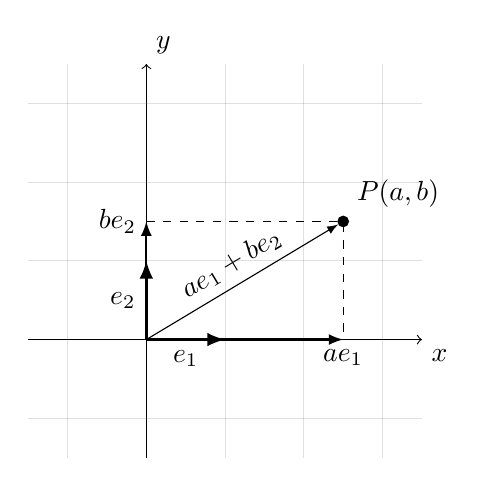
\begin{tikzpicture}[
	point/.style={circle,draw,very thin,fill,inner sep=0pt,minimum size=4pt},
	vector/.style={-latex},
]
	\draw[->] (-1.5,0) to (3.5,0) node[below right] {$x$};
	\draw[->] (0,-1.5) -- (0,3.5) node[above right] {$y$};

	\foreach \x in {-1,1,2,3} {
		\draw[opacity=0.25,gray] (\x,-1.5) to (\x,3.5);
		\draw[opacity=0.25,gray] (-1.5,\x) to (3.5,\x);
	}
	\node[point] at (2.5,1.5) (p) [label=above right:{$P(a,b)$}] {};
	\draw[vector,thick] (0,0) to node[below,at end] {$a\uvec{e}_1$} (2.5,0);
	\draw[vector,very thick] (0,0) to node[below] {$\uvec{e}_1$} (1,0);
	\draw[vector,thick] (0,0) to node[left,at end] {$b\uvec{e}_2$} (0,1.5);
	\draw[vector,very thick] (0,0) to node[left] {$\uvec{e}_2$} (0,1);
	\draw[vector] (0,0) to node[sloped,above] {$a\uvec{e}_1+b\uvec{e}_2$} (p);
	\draw[dashed] (0,1.5) to (2.5,1.5) to (2.5,0);

\end{tikzpicture}
